%%% Preamble starts here.
\documentclass{amsart}
%for the heading
\usepackage{fancyhdr, enumerate,multirow,float}
%for the picture. 
\usepackage{tikz, calc}
%adjust the page width
\usepackage[margin=1in]{geometry}

\usepackage{array}   % for \newcolumntype macro
\newcolumntype{L}{>{$}l<{$}} % math-mode version of "l" column type


%% The next line says how the "vertex" style of nodes should look: drawn as small circles.
\tikzstyle{vertex}=[circle, draw, inner sep=0pt, minimum size=6pt,fill=white]
%%
%% Next, we make a \vertex command as a shorthand in place of \node[vertex} to get that style.
\newcommand{\vertex}{\node[vertex]}

\linespread{1.1}


%special commands for number sets
\def\RR{{\mathbb R}}
\def\NN{{\mathbb N}}
\def\ZZ{{\mathbb Z}}
\def\QQ{{\mathbb Q}}
\def\CC{{\mathbb C}}

% header
\lhead{\sc  Senior Seminar: Homework 11}
\chead{\sc Stefano Fochesatto} 
\rhead{due: Friday 04/17/2020}
\cfoot{}
\pagestyle{fancy}

%%%% Main document starts here.

\begin{document}
\thispagestyle{fancy}
 
\begin{enumerate}
\item (Problem A) Rigorously prove that the relation $R$ (defined both below and on page 40) is an equivalence relation.  \\

Let $G$ be a simple graph with vertex set $V.$ Let $R$ be the relation on $V$ defined as $uRv$ if there exists $\phi \in Aut(G)$ such that $\phi u =v.$ \\

\textbf{Proof:}
Reflexive: (Direct) WTS that for $uRu$. Every automorphism group must contain the identity, which maps every vertex to itself. Therefore $uRu$.\\

Symmetric: (Direct): WTS that if $uRv$ then $uRv$. Suppose $u,v \in V(G)$ such that  $uRv$. By our the definition of $R$ we know that there exists an automorphism $\phi \in Aut(G)$ such that $\phi(u) = v$. Since groups are closed with respect to inverses we know that $\phi^{-1} \in Aut(G)$. Therefore it follows that $\phi^{-1}(v) = u$ and thus $vRu$.\\

Transitive: (Direct) WTS if $uRv$ and $vRw$ then $uRw$. Suppose $u,v,w \in V(G)$, $uRv$ and $vRw$. By our definition of $R$ we know that there exists an automorphism $\phi \in Aut(G)$ such that $\phi(u) = v$ and $\lambda \in Aut(G)$ such that $\lambda(v) = w$. Since $Aut(G)$ is a group closed with respect to function composition we know that $\lambda(\phi) \in Aut(G)$. Note that  $\lambda(\phi(u)) = w$, thus $uRw$.\\

\vspace{1.5in}

\item (Problem B:) A graph that contains a single orbit is called \emph{vertex transitive.} \textbf{Prove} that the regular graph $G_2$ is vertex transitive and $G_4$ is not vertex transitive. \\

\begin{center}
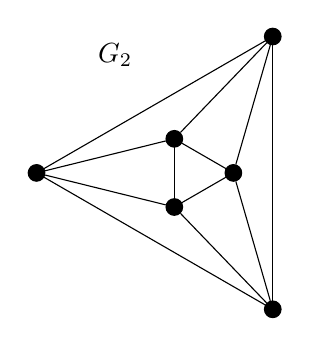
\begin{tikzpicture}
\node at (-1,1.5){$G_2$};
\foreach \i in {0,1,2}{
	\draw (120*\i:.5) -- (120+120*\i:.5);
	\draw (60+120*\i:2) -- (180+120*\i:2);
	\vertex[fill=black] (x\i) at (120*\i:.5){};
	\vertex[fill=black]  (y\i) at (120*\i+60:2){};
	}
\draw (x0)--(y0)--(x1)--(y1)--(x2)--(y2)--(x0);
\end{tikzpicture}
\hspace{1.5in}
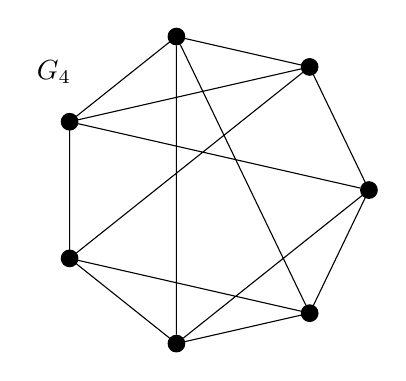
\begin{tikzpicture}
\node at (-2,1.5){$G_4$};
\foreach \j in {0,1,2,3,4,5,6}{
	\vertex[fill=black] (x\j) at (51.43*\j:2){};
	\draw (51.43*\j:2)--(51.43+51.43*\j:2);
	}
\draw (x5) -- (x2) -- (x6)--(x4)--(x1)--(x3)--(x0)--(x5);
\end{tikzpicture}
\end{center}

\textbf{Proof:} Consider the compliments for each graph.

\begin{figure}[H]
\caption{Graph $\overline{G_2}$}
\centering
\includegraphics[width=.35\textwidth]{"figure7".png}
\end{figure}


Consider a vertex $v \in V(\overline{G_2})$. \\
Case 1: WTS: There exists $\phi(v) = u$ such that $u \in N(v)$. Since $\overline{G_2}$ is composed of $3$, $K_2$ components we know that $\phi:(uv)$ must preserve adjacency and non adjacency. Thus $\phi \in Aut(\overline{G_2})$ and from Theorem 2.10 we know that $Aut(\overline{G_2}) \cong Aut(G_2)$ thus $\phi \in \overline{G_2}$.\\


Case 2: WTS: There exists $\phi(v) = u$ such that $u \in \overline{N(v)}$. Note $\overline{G_2}$ is composed of $3$, $K_2$ components. Let $w \in N(v)$ and $x \in N(u)$. Consider the mapping $\phi:(vu)(wx)$. Note that $N(\phi(v)) = w$, $N(\phi(v)) = x$ therefore adjacency and non adjacency is preserved. Thus $\phi \in Aut(\overline{G_2})$ and from Theorem 2.10 we know that $Aut(\overline{G_2}) \cong Aut(G_2)$ thus $\phi \in \overline{G_2}$.\\

\begin{figure}[H]
\caption{Graph $\overline{G_4}$}
\centering
\includegraphics[width=.35\textwidth]{"figure8".png}
\end{figure}

Note that $\overline{G_4}$ has two components a $C_4$ and $C_3$. Let $u \in C_4$ and $v \in C_3$. Note that any mapping with the permutation $(uv)$ would fail to preserve $total distance$ for either vertex. Thus $\overline{G_4}$ is not vertex transitive. From Theorem 2.10 we know that $Aut(\overline{G_4}) \cong Aut(G_4)$ and therefore $G_4$ cannot be vertex transitive. 






\vspace{1.5in}


\item (Problem C) For which pairs $k$ and $n$ of positive integers with $k \leq n$ does there exist a graph $G$ of order $n$ having $k$ orbits?\\

\textbf{Proof:} 

Algorithm 1:
Consider the tuple $(k,n)$ where $k = n \geq 6$. Now I will describe an algorithm which produces a graph $G$ for which the tuple applies.\\
Input: A tuple $(k,n)$ where $k = n \geq 6$.\\
Initialization: Consider the graph $G$, for which the tuple $(6,6)$ applies.
\begin{figure}[H]
\caption{}
\centering
\includegraphics[width=.5\textwidth]{"figure1".png}
\end{figure}
Iteration: If $(k,n)$ doesn't apply append a vertex to the graph, incident to the leftmost vertex. 
\begin{figure}[H]
\caption{}
\centering
\includegraphics[width=.5\textwidth]{"figure2".png}
\end{figure}
Note that the graph now corresponds to the tuple $(7,7)$. Thus the algorithm will terminate after $n-6$ iterations and produce a graph that corresponds to the $(k,n)$ tuple. Thus all same number tuples greater than 5 apply. \\\\


Algorithm 2:
Now consider the tuple, $(k,n)$ where $n > k$ and $k \geq 6$. Now I will describe an algorithm which produces a graph $G$ for which the tuple applies.\\
Input: A tuple (k,n) where  $n > k$ and $k \geq 6$.\\
Initialization: Consider the graph $G$ with $m$ orbits and $i$ vertices. Note that $(6,7)$ applies to $G$.
\begin{figure}[H]
\caption{}
\centering
\includegraphics[width=.5\textwidth]{"figure3".png}
\end{figure}
Iteration: if $m \neq k$ append a vertex to the graph, incident to the leftmost vertex.
\begin{figure}[H]
\caption{}
\centering
\includegraphics[width=.5\textwidth]{"figure4".png}
\end{figure}
Note that $G$ now has $m+1$ orbits and, $i+1$ vertices. This part of the algorithm, terminates after $k-6$ iterations and produces a graph with $k$ orbits and $m = i+k-6$ vertices. \\\\
Iteration 2: Add trivial components to $G$ until $m = n$. Note that adding these vertices does not add to the number of orbits yet increases the number of vertices. Finally the algorithm terminates when $m = n$ and produces a graph which corresponds to the tuple $(k,n)$.\\
For example when we input the tuple $(6,9)$ the algorithm produces the following graph,
\begin{figure}[H]
\caption{}
\centering
\includegraphics[width=.5\textwidth]{"figure5".png}
\end{figure}
So we have shown that we can produce a graph for every tuple $6\leq k,n \leq \infty$. There are more and I think they require special cases like $(1, n)$ which corresponds to $K_n$ or $\overline{K_n}$.
\\\\
P.S: I did exactly what you suggested in your email, and I saw a few patterns but not any that would produce an algorithm regardless of the choices for $k$ and $n$. Describing how to produce a graph for when $2 \leq k \leq 5$ was difficult even though through exploring those graphs I know that tuples like $(2,2),(3,3),(4,4)$, and $(5,5)$ don't exist. Also when I discussed this question with a group of other students the idea of allowing multi-graphs came up but I felt that it would make the problem too trivial. A pattern I found that was really interesting is that we can prove the tuple $(k,k+1)$ exists by induction on $k$ starting on $k = 2$ by picking the graph that uses a trivial component, taking the compliment and then adding a trivial component. 








\vspace{1.5in}
 

\item (Problem D) For which pairs $k$ and $n$ of positive integers with $k \leq n$ does there exist a graph $G$ of order $n$ and a vertex $v$ of $G$ such that there are exactly $k$ vertices similar to $v$? (Recall that $u$ and $v$ are \emph{similar} if $v$ is in the same orbit as $u.$\\

\textbf{Proof:} Consider a tuple $(k,n)$ of positive integers with $k \leq n$. Take $k$ vertices and construct a $K_k$, let the rest of the $n-k$ vertices be trivial components. This construction produces a graph for every tuple except $(1,n)$ since any $K_1$ would be included in the orbit of trivial components. To construct a graph for the tuples $(1,n)$ consider a $K_{n-1}$ and a single trivial component. This construction produces a graph for every tuple $(1,n)$ except for $(1,2)$ since $K_{2-1} = K_1$ and thus any graph on 2 vertices must have an orbit with 2 elements. Therefore, with the exception of $(1,2)$ there exists a graph for every tuple $(k,n)$ where $k \leq n$.
\vspace{1.5in}
 


\item (Problem E)  On page 44, the text graphs the Cayley color graph of the group $S_3$ with generators $\alpha=(123)$ and $\beta=(12).$ Determine (i.e. draw the graph of...) the Cayley color graph of the group $S_3$ with generators $\beta=(12),\: \gamma=(23),$ and $\delta=(13)$. Prove that the automorphism group of this graph is isomorphic to $S_3.$\\

\textbf{Proof:} First note that we can get the permutation $(132)$ by the following compositions: $(12)(23)$, $(13)(12)$, and $(23)(13)$. We can get the permutation $(123)$ by the following compositions: $(23)(12)$, $(12)(13)$, and $(13)(23)$. Note that every permutation in $\Delta = \{(12),(23),(13)\}$ is order two and thus every edge in $D_\Delta(S_3)$ is bi-directional. Thus the following graph $D_\Delta(S_3)$ is,

\begin{figure}[H]
\caption{}
\centering
\includegraphics[width=.35\textwidth]{"figure6".png}
\end{figure}

By Theorem 2.14 we know that the color preserving automorphism group of $D_\Delta(S_3)$ is isomorphic to $S_3$.

\vspace{1.5in}



\end{enumerate}

\end{document}
